\documentclass[conference]{IEEEtran}

% correct bad hyphenation here
\hyphenation{op-tical net-works semi-conduc-tor}
\usepackage{graphicx}
\usepackage{float}
\begin{document}
\title{Kappa: A Synchronized Video Viewer}

\author{\IEEEauthorblockN{Zhan Xiong Chin}
\IEEEauthorblockA{chinz@seas.upenn.edu\\
Univ. of Pennsylvania\\
Philadelphia, PA}
\and
\IEEEauthorblockN{David Liao}
\IEEEauthorblockA{liaod@seas.upenn.edu\\
Univ. of Pennsylvania\\
Philadelphia, PA}
\and
\IEEEauthorblockN{Yoo Jin Kim}
\IEEEauthorblockA{yoojkim@seas.upenn.edu\\
Univ. of Pennsylvania\\
Philadelphia, PA}
}



% make the title area
\maketitle

% As a general rule, do not put math, special symbols or citations
% in the abstract
\begin{abstract}
  E-sports is a market that is rapidly becoming popular and widespread, yet often does not see high quality software solutions catering to it. Professional e-sports teams, whose members typically play remotely, do not have good ways to analyze or review their games together. Instead, they rely on ad-hoc solutions using a combination of existing software, leaving considerable room for improvement.

  To address this need, we propose Kappa, a synchronized all-in-one video viewing platform that allows e-sports teams to view, annotate, and analyze video replays of games remotely. The main technical contribution is designing both a scalable backend that supports our custom syncing protocol as well as pioneering a frontend UI that solves existing complications that arise when integrating with other third party systems. We achieved the creation of a fluid and responsive UI that is intuitive and integrates well with Youtube. With scalability and cost in mind, the UI is designed to complement the backend by helping minimize server-side upstream communication. The backend architecture emphasizes flexibility and reliability, with communication latencies of less than 100ms to all clients under all loads using techniques that exploit differential payloads and minimize overhead communication costs.
\end{abstract}

\IEEEpeerreviewmaketitle

\section{Introduction and Problem definition}

  E-sports is a rapidly growing market, with a burgeoning number of professional teams such as Evil Geniuses or Fnatic entering the field in games such as DOTA 2 or League of Legends to compete for multi-million dollar prize pools in online and offline competitions. With so much at stake, these professional teams spend a considerable amount of their time practicing and attempting to improve their skills. For instance, a typical day for a professional player would be to spend the morning playing a number of matches, then reviewing their video replays as a team in the afternoon. Similar to athletes in other sports, any improvements to the training process can yield significant impact on their success rates.

  However, despite the importance of such training and analysis time, the processes that teams use for these are often woefully inadequate. Unlike a conventional professional sporting team, e-sports teams are often decentralized in nature, with their members potentially being in completely different cities or countries for most of the year. Thus, any shared analysis time tends to rely on ad-hoc solutions. For example, a team might communicate via multiple screen shots edited with Microsoft Paint, or by manually communicating to each other the relevant video timings in a video replay. Such ad-hoc solutions slow down the analysis process and significantly increase the chance of a miscommunication, while making it difficult to remember the details of a previous analysis session.

\section{Solution outline}

\subsection{Overview}

  Our proposed solution to this need is Kappa, an all-in-one web platform that aims to make collaborative video analysis sessions easy to run. Our platform allows videos to be loaded from YouTube, synchronizing their playback across multiple browsers. A shared canvas overlaid across the videos allows for annotations and other details to be easily communicated to the other users of the platform.

\subsection{Typical work flow}

  A typical work flow for our platform is as follows:

  \begin{enumerate}
      \item The team captain of an e-sports team selects a number of video replays for an analysis session. These can either be publicly available video replays of professional games on YouTube, or video replays of the team's own games. In the latter case, the team captain would upload them to YouTube first.

      \item The team captain copies the YouTube link into our platform's room creation form, creating a room with the relevant video in it.

      \item The team captain invites his teammates (from his friends list in our platform) to the newly created room.

      \item The team watches through the video. Actions such as fast-forwarding/rewinding, pausing/playing, volume changes, or changing the video or the video time are synchronized across all clients automatically.

      \item The team also can draw or write annotations on the video. For example, a team member might circle a location inside the video of the game, while describing some strategic maneuver to his teammates. To do this, the relevant team member opens the drawing tool bar at the side of the video, then uses the provided tools to draw or write his annotations directly onto the video.

      \item Once the team finishes the analysis session, they may wish to review any of the annotations made during that session at a later time, which they can do by opening up the "previous sessions" link on our platform.
  \end{enumerate}

\subsection{Architecture}

  \begin{figure}[H]
      \centering
      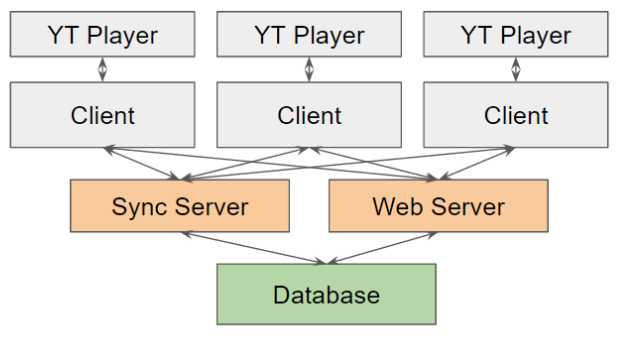
\includegraphics[width=\linewidth]{figure1.PNG}
      \caption{Architecture Layout}
      \label{fig:my_label}
  \end{figure}

  The main web server of the platform is in charge of handling login and account registration processes. It is hosted using a custom server written in Go. It also allows the user to create rooms (each room is a single shared video instance) and invite friends and teammates to join the relevant room. All data is stored in an SQL database.

  The synchronized video viewer is in charge of tracking changes to the video's state (play/pause, volume, current playback time) and sending them to the sync server (described below). It is built in JavaScript and React on top of the YouTube IFrame Player.

  The shared canvas provides a layer on top of the video which allows for annotations and drawings to be overlaid over the video. Any drawing or annotation made on the canvas is immediately synchronized with other clients via the sync server as well. It is also built in JavaScript and React.

  The sync server is in charge of passing messages back and forth between the various clients to synchronize their video and canvas state. It is also written in Go and relies on WebSockets to provide a reliable and high-performance communication channel between itself and its clients.

\section{Design decisions}

\subsection{Video Player}

  Our video player underwent 3 distinct iterations. We will describe the benefits and drawbacks of each iteration in some detail, as well as the evaluation criteria that led us to finally choose the last iteration as our main video player component. The iterations were:

  \begin{enumerate}
      \item Combined HTML5 canvas video player
      \item Separate video player element
      \item YouTube player
  \end{enumerate}

  Initially, our video player was combined with our HTML5 canvas drawing elements, directly manipulating the pixels in the canvas with video frames. While this provided us the ability to introduce additional effects into the video (e.g. blur effects or gamma correction), these were not useful features for our end users, who did not need any advanced video editing effects, but rather improved communication tools.

  Thus, in our second iteration of the video player, for simplicity and modularity of design, we split the video player into a standalone HTML5 video component. However, for both these iterations, to handle the main use case of our project, we had to implement our own video hosting platform. After further conversations with potential users, and consideration of our ability to scale a video hosting platform, we decided that a better choice would be to make use of YouTube's embedded player API instead, and extend our own functionality over that.

  Making use of the YouTube player rather than writing our own player enables users to more easily make use of existing video resources such as previously hosted YouTube videos. This not only leverages YouTube's high performance content delivery network across all users viewing the same video, but also makes it easy for teams to analyze video replays from other competitions or tournaments, which are frequently posted to YouTube.

  The trade-off for this decision is that we do not have the same granularity when tracking the video state, leading to minor delays in responsiveness of the synchronization. Unlike most of e-sports and gaming, video viewing and analysis are not heavily time-sensitive, thus we deemed this delay in response tolerable, as long as throughput and reliability were maintained.

  Another minor trade-off was the development time needed to adapt our code to the new player. This was significantly mitigated by the modular design of our code. The video player was implemented in its own React component, allowing the change to be made quickly and efficiently with almost no impact on the rest of the code base.

\subsection{Canvas drawing behavior}

  The interaction between our two main front-end components, the video player and the canvas, offered multiple option
s, of which the best choice was not initially clear. For instance, a small sample of the multiple possible behaviors we brainstormed are listed below:

  \begin{enumerate}
    \item The canvas and the video could be completely separate. Drawings on the canvas would be unaffected by the time listed in the video, only disappearing when erased.

    \item Drawings on the canvas could be temporary, disappearing a fixed number of seconds (e.g. five seconds) after being drawn. They would be unaffected by video playback.

    \item The ability to draw on the canvas would only be enabled when the video was paused, disappearing once the video is played again.

    \item Drawings on the canvas would be permanent until erased, but would be "tagged" to a specific video timing, reappearing if the video was played through the same time.

    \item Drawings on the canvas would be tagged to a specific video timing, only appearing when the video is playing at that time.
  \end{enumerate}

  To resolve this issue, we approached the problem in three ways. Firstly, we made a list of use cases for the drawing feature, then established properties that the drawing behavior should display based on each use case. Secondly, we implemented the most compelling behaviors we thought of, then used it ourselves for a brief period to see how intuitive the interactions would be. Thirdly, we examined the technical features and trade-offs (e.g. performance, memory required) needed for each behavior, using this information to supplement our design decision.

  As an example of the first approach, one use case we came up with was for a user to circle a moving character on screen to draw attention to the character's position in the game. Analyzing this use case suggests that any permanent drawing not tied to a specific time in the video is intuitively unsatisfactory: the circle would be redundant at any other point in time. However, if the video is paused, the drawing should remain for as long as desired. Additionally, it would be preferred for a drawing to reappear if the video is rewound to the same point in time, as a reminder to the idea communicated. Furthermore, if a user decides that the annotation or drawing is no longer relevant to that point of the video, there should be an easy way to delete it from the playback.

  Based on this and the other two approaches listed, we eventually settled on the last option listed above: having drawings on the canvas tagged to a specific video timing. More concretely, we store drawings as a free-form collection of pixels, with each pixel recording the starting and ending time that it appears on the video. Initially, when a pixel is created, the pixel's starting time is tagged to the video time where it was drawn, with the ending time tagged to a fixed number of seconds after its starting time. This exhibits both the desired play and pause behavior we want, as well as the ability for drawings to reappear when a video is rewound back to the same time. This also makes erases easy to handle: if a pixel is erased, we just set its ending time to the video time-stamp where it was erased.

  Looking at the technical aspect of this choice, it does not increase bandwidth significantly, since we need to send either per-pixel or per-stroke information regardless of which method was chosen. On the other hand, it does have the potential to impact performance, since now fast-forwarding, rewinding, etc. need to make look-ups against the entirety of the canvas pixel data across the entire video. Despite this concern, testing revealed that it was not a significant factor. We note that in the future, if need be, further optimizations can be made either by improving the data structures which store the canvas data, or by adding GPU acceleration to the canvas (each pixel can be treated individually from any other pixel, which is ideal for a GPU-based speedup).

\section{Technical depth}

    Aside from the design decisions listed above, other parts of our project which we designed and implemented from scratch are described below.

\subsection{Syncing Backend}

    We home-brewed a publisher-subscriber system to handle the syncing of player states. In order to ensure a smooth user experience, the syncing servers maintained a direct connection between all users via WebSocket connection. Using WebSockets as our main communication channel ensures both speed (as opposed to a method such as long polling) and reliability in our communications. While a connectionless protocol such as UDP may be even faster (though less reliable), we are not able to make use of it via a web application, leaving WebSockets as the highest performance option available to a majority of web users.

    Each user that joins a room is assigned to a server that manages several rooms. This abstraction improves our scalability, as our system can assign new rooms to the least loaded (i.e. lowest user count or lowest activity) server.


\subsection{Data Representation}

    Every room's state can be summarized into three main parts, the current list of users, the video state and the canvas state. Based on our current user case, neither the list of users nor the video state require any special optimizations to represent. For instance, when a new user joins, the back-end server just needs to send a message to all clients to update their list of active users.

    However, as mentioned above, the canvas state took a considerable amount of tweaking and experimentation to come up with an intuitive design. As described in the Design Decisions section, we represent the canvas by having each pixel that is drawn to the canvas have a starting and ending time (as well as a color). Thus, on each client, as well as the back-end server, we store the canvas as a hash map of pixel locations to a list of pixels. Our free-form drawing tool just converts each line segment drawn to a list of pixels, and sends those pixels over to the other clients via the server. Since a new pixel just needs to be appended to the correct list in constant time, our front-end system is highly responsive to new changes coming over the network.

    One thing to note with this data representation is that at any given point in time, the cost to figure out what color (if any) a given pixel is requires searching the entire set of drawn pixels at that location over all possible times. While we considered optimizing this by using a segment tree data structure, our benchmarks suggested that for a typical load, most pixel locations will not have more than tens (or at most even a few hundred) of pixels, so such an optimization would not produce a significant speed-up.

\section{Evaluation of solution}
    Over the course of this project, every iteration is preceded and followed by a series of feedback from external sources. Since the project is created with users in mind, we wanted to ensure that our work is guided by their input. Additionally, there is an equal emphasis on performance since our product is highly interactive. Therefore, the project has the following metrics for success: instrumentation on the front-end for latency, user evaluation, and constructive feedback. Note that the data is gathered on a Windows 10 Intel Core i7-6700K @ 4.00 GHz with a AMD Radeon R9 Fury Series.



\subsection{Instrumentation}
    We used existing libraries such as stats.js as well as browser debuggers to measure our component's performance. To ensure the most fluid user experience, we need to render the canvas state at an average of 60fps. In figure 2 we benchmark the resting performance of our component when it is only rendering the video and any existing drawings. Averaging at 73.2 fps, we are well above the 60 fps baseline. In figure 3, we benchmark the active performance of our component when it is both rendering and updating state. This simulating heavy user load, which averages at 69.8 fps. Again, we float above the target fps despite the drop of 3.3 fps in average fps.

    \begin{figure}[H]
      \centering
      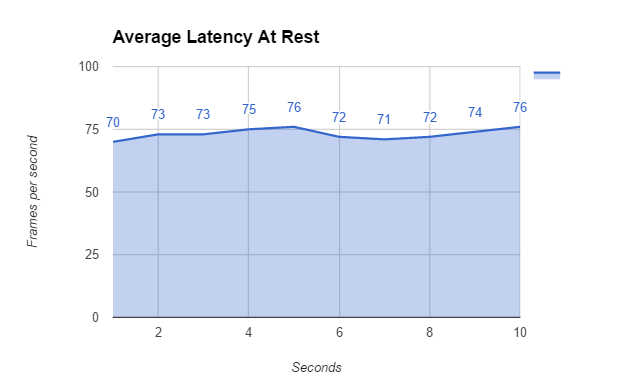
\includegraphics[width=\linewidth]{figure2a.PNG}
      \caption{}
      \label{fig:my_label}
    \end{figure}

    \begin{figure}[H]
      \centering
      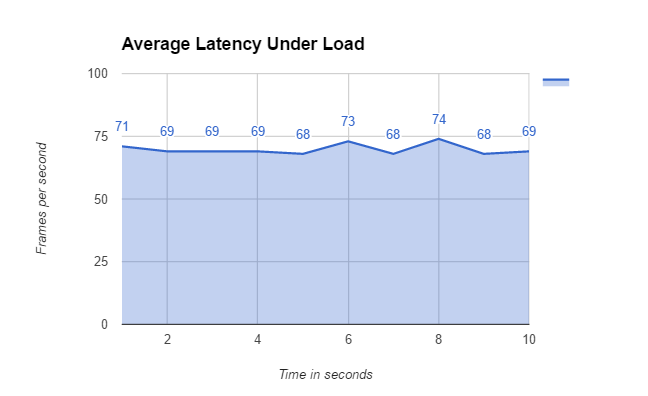
\includegraphics[width=\linewidth]{figure2b.PNG}
      \caption{}
      \label{fig:my_label}
    \end{figure}

    We experimented with various payload representation and sizes. In one variation, we would send over a list of changed pixels, whereas in another, we sent over line segments (a pair of Cartesian coordinates) and defer calculation to the client. In figure 4 and 5, we benchmark each result to determine which protocol to ultimately settle on. It turns out that the overall cost incurred by the size and computation trade-off is insignificant when compared to the cost of simply streaming and decoding video. Thus the representation was inconsequential and we decided to use list of changed pixels for simplicity.

    \begin{figure}[H]
      \centering
      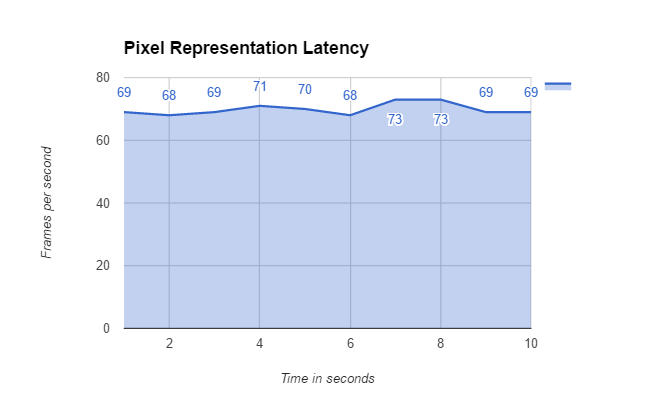
\includegraphics[width=\linewidth]{figure3a.PNG}
      \caption{}
      \label{fig:my_label}
    \end{figure}
    \begin{figure}[H]
      \centering
      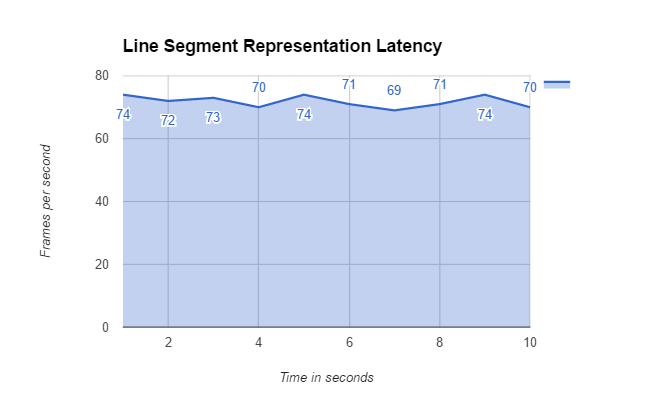
\includegraphics[width=\linewidth]{figure3b.PNG}
      \caption{}
      \label{fig:my_label}
    \end{figure}

    The final metric we used to determine performance is network response time. We simply measured the time it took for a change to reflect on another machine. In this case, we consider the joint timing of both the canvas state as well as the video state and take the longest of both times. Figure 6 shows the latencies over 10 separate requests.

    \begin{figure}[H]
      \centering
      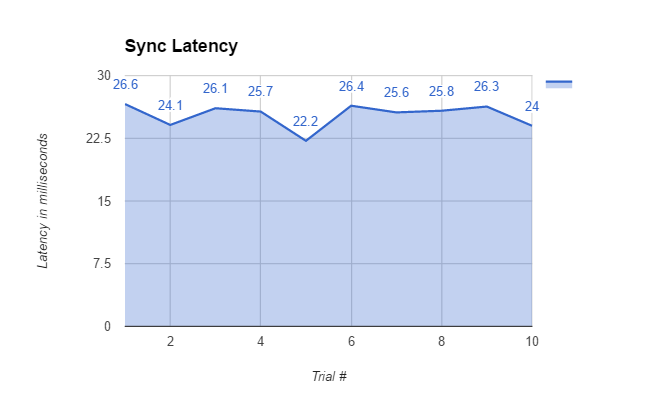
\includegraphics[width=\linewidth]{figure4.PNG}
      \caption{}
      \label{fig:my_label}
    \end{figure}

\subsection{User Feedback}
    We constructed a series of questions that we thought will give us the best understanding of how to iterate on our product. We then reached out to users and presented them with a series of questions prior to using the product and after using them. The series of questions given prior to using the product were meant to gauge general user needs for the product. These included questions that addressed what challenges users might have in a certain area of collaborative work or video watching. We then presented post-demo questions that addressed what challenges users had with the product. This was a guided back and forth interview about how the product can be improved.

    In order to obtain unbiased feedback, our users were given a specific task but no further instruction as to how it would be executed. For example, we asked our users to create a new room from the home page and observed to see if there was any confusion in the UI that would make it unintuitive.

\section{Implications of Project}

    Two ethical concerns exist as our platform grows at scale. Though these concerns are important no matter of the scale, it would be more prominent as the scale grows.

    First concern is on copyright issue of contents that are being streamed in each room. As users stream more contents, copyright of each content can be an issue. Though there are no functionality to directly detect copyright violation, since users have to provide the YouTube link of the video to stream it, any videos that became unavailable on YouTube due to copyright issues would not be able to be streamed on our platform.

    Second concern is regarding content of things written by viewers. Since users have unrestricted ability to use canvas system, content of things that can be written by users cannot be controlled. And as the number of users grow, there might be malicious usage of canvas functionality by some users. Our main approach here is to restrict the process for the users to join rooms so that any unidentified viewers cannot join the room. We are furthermore thinking of ways to restrict the ability of users to write on canvas, for instance, by limiting the amount of ink each user has.
\section{Future work}

    While our current solution is fairly capable of solving the problem that we posed in the introduction, we foresee numerous improvements that can still be made, and hope to continue development in these areas. Based on suggestions by potential end-users, the following lists some potential steps that can be pursued.

\subsection{Front-end development}

    Simple tweaks that would improve the experience including the addition of even more annotation and drawing tools, to allow users to have a greater variety of methods to communicate important information to their teammates. Additional communication channels such as built-in voice chat would also improve the user experience by removing the need to use third-party tools for this while on our platform.

\subsection{Back-end development}

    While our platform currently handles small to moderate loads well (e.g. 5-20 people in a room, reflecting the average size of an e-sports team), it may be worthwhile to extend our platform to support operations at a larger scale. For instance, the platform currently is untested for an extremely large number of rooms. In addition, there is potential to expand our platform for general video game streaming, which would require on the order of up to thousands of viewers per room.

    Another extension that would serve our use case well would be to introduce a more fine-grained permission system into our room structure. For instance, the captain of an e-sports team might want to be the only one who has annotation and drawing capability for most of a session, while still allowing teammates to toggle the playback as desired. This feature would also be useful for other extensions outside of e-sports (described below).

\subsection{Extension to a different target demographic}

  Furthermore, despite our focus on the gaming and e-sports market, our platform is fairly general in nature. We can foresee numerous use cases outside of e-sports, even with minimal tweaks to the system.For example, a non-exhaustive list of other potential use cases is listed here:

  \begin{enumerate}
      \item Movie/Video editing and annotation, providing a platform for members of a film production or review team to work collaboratively.

      \item Shared movie or TV watching, providing a means for remote friends to share such an experience together at the same time.

      \item A virtual classroom setting, with a teacher teaching via video stream while making use of the annotation feature to easily communicate information to students.
  \end{enumerate}

   Considering this, there may be value in converting part of the functionality into a general-purpose library, so that other developers can easily extend and modify our project to better suit the needs of other users.

\section{Conclusion}

  In conclusion, we have built an easy-to-use and scalable solution that solves an existing need in the e-sports industry. Through our platform, members of remote e-sports teams now have a responsive and intuitive method for analyzing video replays with their teammates. Our benchmark results suggest that the platform is fairly performant at typical loads, though further testing and usability studies can still be done to improve the accuracy of the results. In addition, as described above, the platform is fairly general-purpose and extensible to a good number of alternative use cases. We hope to continue working on the project and adding more useful features as desired by our users.

% use section* for acknowledgment
\section*{Acknowledgment}
We would like to thank our senior design advisor Professor Boon Thau Loo for the invaluable support and advice that he has provided us throughout this project.

% TODO: don't forget to add/edit our references section

% trigger a \newpage just before the given reference
% number - used to balance the columns on the last page
% adjust value as needed - may need to be readjusted if
% the document is modified later
%\IEEEtriggeratref{8}
% The "triggered" command can be changed if desired:
%\IEEEtriggercmd{\enlargethispage{-5in}}

% references section

% can use a bibliography generated by BibTeX as a .bbl file
% BibTeX documentation can be easily obtained at:
% http://mirror.ctan.org/biblio/bibtex/contrib/doc/
% The IEEEtran BibTeX style support page is at:
% http://www.michaelshell.org/tex/ieeetran/bibtex/
%\bibliographystyle{IEEEtran}
% argument is your BibTeX string definitions and bibliography database(s)
%\bibliography{IEEEabrv,../bib/paper}
%
% <OR> manually copy in the resultant .bbl file
% set second argument of \begin to the number of references
% (used to reserve space for the reference number labels box)
\begin{thebibliography}{1}

\bibitem{IEEEhowto:kopka}
H.~Kopka and P.~W. Daly, \emph{A Guide to \LaTeX}, 3rd~ed.\hskip 1em plus
  0.5em minus 0.4em\relax Harlow, England: Addison-Wesley, 1999.

\end{thebibliography}


\end{document}
